% !TeX spellcheck = de_DE

\chapter{Methodology}
\label{chap:k2}

The following sections introduce the principles of 3D lane marking reconstruction method as well the materials used in this work.% sorting with respect to their position in the processing chain (Fig.1.).

~\cref{sec:Materials} gives the information of the input dataset and some preprocessing applied in this work.~\cref{sec:LineExtraction} describes the standard line detection algorithm for automatic lane marking extraction.~\cref{sec:Geometry} introduces the geometric properties of aerial images and their mathematical models, including collinearity equation and lens distortion correction.

~\cref{sec:LineFitting} presents the principle of line fitting and further derives the non-linear LS model for line equations in two-points form.~\cref{sec:LSadj} elaborates the usage of line fitting on 3D lane marking reconstruction, where the observations are in image space yet the unknowns in object space. It is the key approach to solve non-textured-neighborings quasi-infinite line reconstruction problem. As initial values of unknown quantities are required in non-linear LS model, the extracted line features are projected onto DSM to provide 3D lane marking approximations in ~\cref{sec:LineProjectionOnDSM}.

% mainflowchart [!hb]
Fig. 1. Work flow

\clearpage

%%%%%%%%%%%%%%%%%%%%%%%%%%%%%%%%%%%%%%%%%%%%%%%%%%%%%%%%
\section{Materials}
\label{sec:Materials}

% subflowchart-preprocessing of input data

\paragraph{Aerial Images}

For real-time mapping applications during disasters, mass events and traffic monitoring scenarios, the German Aerospace Center (DLR) has developed a new optical sensor system-- the 4k system-- on a helicopter. %[F. Kurz et al.]
The low-oblique aerial images used in this work are acquired from Canon EOS 1D-X, one of the non-metric cameras in 4k system, with an oblique viewing angle of 15$\degree$ and around 500m flying height above ground.

An example aerial image is shown in~\cref{fig:OriImg}.~\cref{tab:CameraProperties} lists the properties of this camera, and~\cref{tab:SensorViewingGeometry} provides the viewing geometry information.
\newline

\begin{table}[!h]
  \centering
  \begin{tabular}{ll}
  \toprule
                                      {} & \textbf{Canon EOS 1D-X} \\
  \midrule
  Lenses                          & Zeiss Makro Planar 2/50\\
  \\[-1em]
  Sensor / Pixel size             & Full frame CMOS / 6.944 \textmu m\\
  \\[-1em]
  \multirow{2}{*}{Image size}     & 5184$\times$3456 pixel, ratio 3:2\\
                                  & (17.9 MPix)\\
  \\[-1em]
  ISO                             & 100--204800\\
  \\[-1em]
  max. frame rate / max. images   & 14 fps/ 180 images\\
  \\[-1em]
  Exposure time                   & 30 s -- 1/8000 s\\
  \\[-1em]
  Data interface                  & LAN (EDSDK software interface)\\
  \bottomrule
  \end{tabular}
  \caption{Properties of the oblique camera }
  \label{tab:CameraProperties}
\end{table}

\vspace*{1 cm}

\begin{table}[!h]
  \centering
  \begin{tabular}{lll}
  \toprule
                         & \textbf{RGB, 50mm lens} \\
  \midrule
  Viewing directions     & $\pm$15$\degree$\\
  \\[-1em]
  \multirow{2}{*}{FOV}   & $\pm$34$\degree$ across strip,\\
                         & $\pm$13$\degree$ along strip\\
  \\[-1em]
  Coverage @500m         & 780 m $\times$ 230 m\\
  GSD      @500m         & 6.9 cm (nadir)\\

  \bottomrule
  \end{tabular}
  \caption{Viewing geometry}
  \label{tab:SensorViewingGeometry}
\end{table}

\clearpage

The images are acquired with a special flight configuration at both sides of the motorway which guarantees a stereo view perpendicular to the lane marking direction. This is realized by flying at the right-hand side with respect to flying direction along the motorway, with the left oblique camera looking left-down to the motorway, in both forward and backward trip. The flight configuration is shown in~\cref{fig:FlightTrajectory} on Google Earth platform.

\begin{figure}%[!h]
  \centering
  \subfloat[]{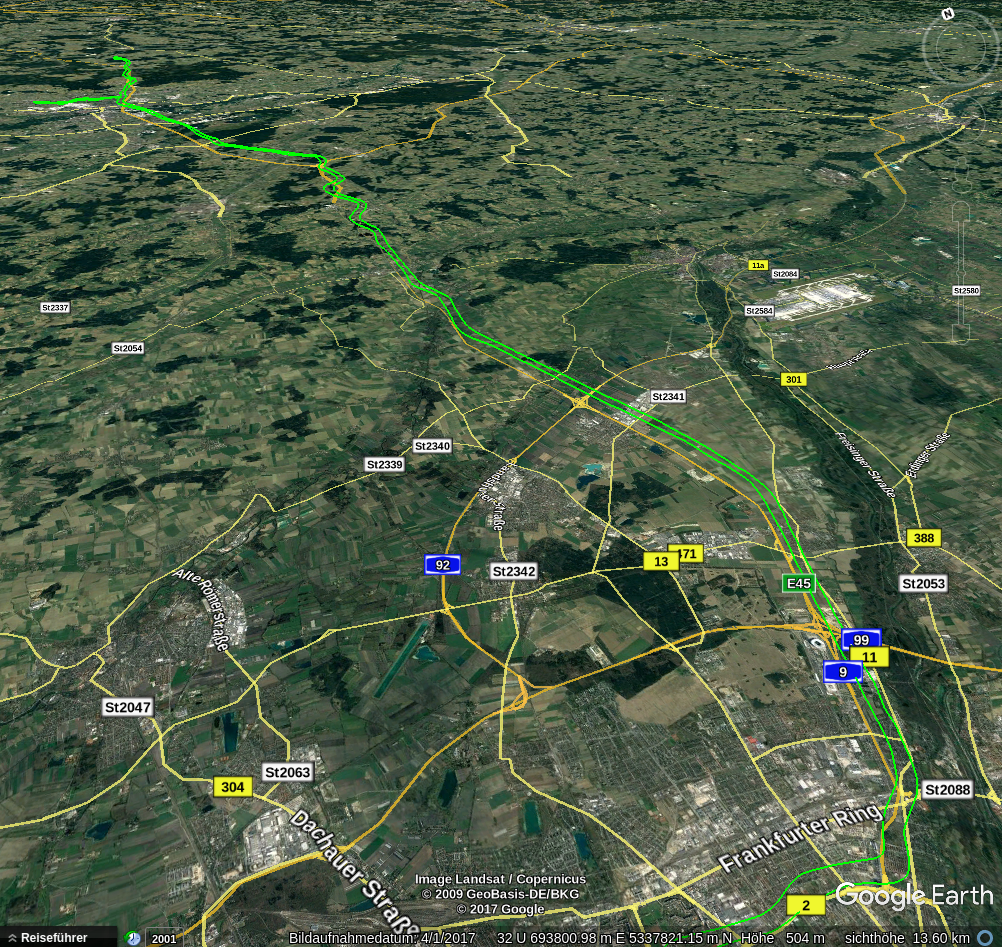
\includegraphics[height=0.45\textwidth]{FlightTrajectory5.png} \label{fig:trajectory1}}
  \subfloat[]{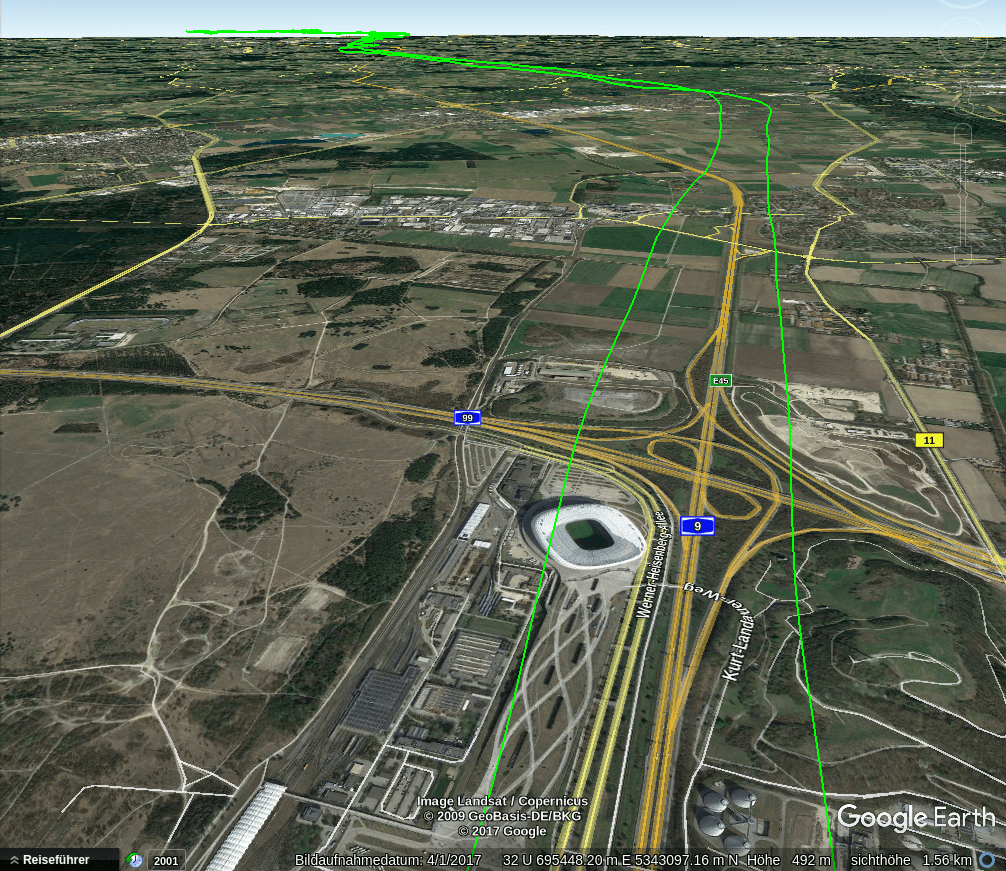
\includegraphics[height=0.45\textwidth]{FlightTrajectory3.png} \label{fig:trajectory2}}
  \caption{Flight Trajectory on Google Earth platform. The green polyline shows the flight trajectory.}
  \label{fig:FlightTrajectory}
\end{figure}


\paragraph{Image Orientations}
The image orientations are refined by GPS-assisted self-calibrating bundle adjustment.
The achieved accuracies are shown in~\cref{tab:EOaccuracy} and~\cref{tab:IOaccuracy}.

% table here!!! 
\begin{table}[!h]
  \parbox{.45\linewidth}{
    \centering
    \begin{tabular}{ll|ll}
    \toprule
    \multicolumn{4}{c}{Exterior Orientations} \\
    \midrule
                &[meter] &                  & [degree]\\
    \hline
    $\sigma_X$  & 123    & $\sigma_{Roll}$  & 123\\
    $\sigma_Y$  & 123    & $\sigma_{Pitch}$ & 123\\
    $\sigma_Z$  & 123    & $\sigma_{Yaw}$   & 123\\
    \bottomrule
    \end{tabular}
    \label{tab:EOaccuracy}
    \caption{EO Accuracies}
  }
  \hfill
  \parbox{.45\linewidth}{
    \centering
    \begin{tabular}{ll}
    \toprule
    \multicolumn{2}{c}{Interior Orientations} \\
    \midrule
                &[meter]\\
    \hline
    $\sigma_X$  & 123\\
    $\sigma_Y$  & 123\\
    $\sigma_Z$  & 123\\
    \bottomrule
    \end{tabular}
    \label{tab:IOaccuracy}
    \caption{IO Accuracies}
  }
\end{table}

% The undistorted images can be further derived with the calibrated lens distortion parameters.

\paragraph{\gls{dsm}}
A disparity map is firstly generated from the aerial images using \gls{sgm} algorithm and then reprojected into a DSM of 0.2 m grid spacing with the bundle-adjusted orientations.

\paragraph{Orthorectified Images}
With the bundle-adjusted image orientations, the original images are pixel-wise reprojected onto DSM model to generate the orthorectified images, as shown in~\cref{fig:OrthoImg}.
orthophoto characteristics:
georeferenced

\paragraph{Road Masks}
Road segments are masked out from original images based on \gls{osm} data: Firstly, OSM data is written into orthorectified images. Road regions are then extracted with 25 meter buffer width around road axes. By back-projecting the mask from orthorectified image to original image, it can then be used to mask out the road regions on the original images, as shown in~\cref{fig:MaskedImg}.

\begin{figure}%[!h]
  \parbox{.45\linewidth}{
    \centering
    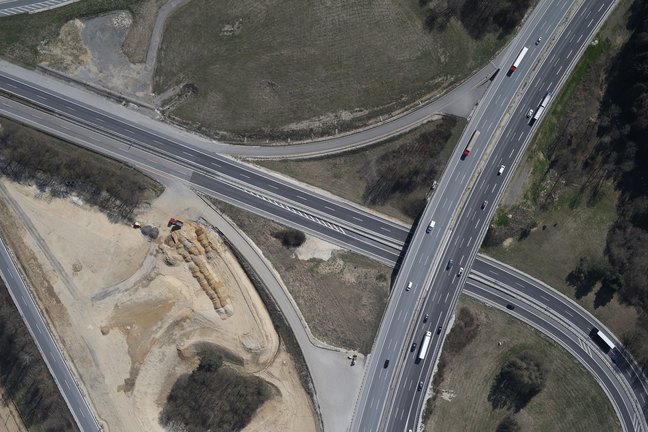
\includegraphics[width=0.45\textwidth]{L1234_rsz.png}
    \caption{Original Image}
    \label{fig:OriImg}
  }
  \hfill
  \parbox{.45\linewidth}{
    \centering
    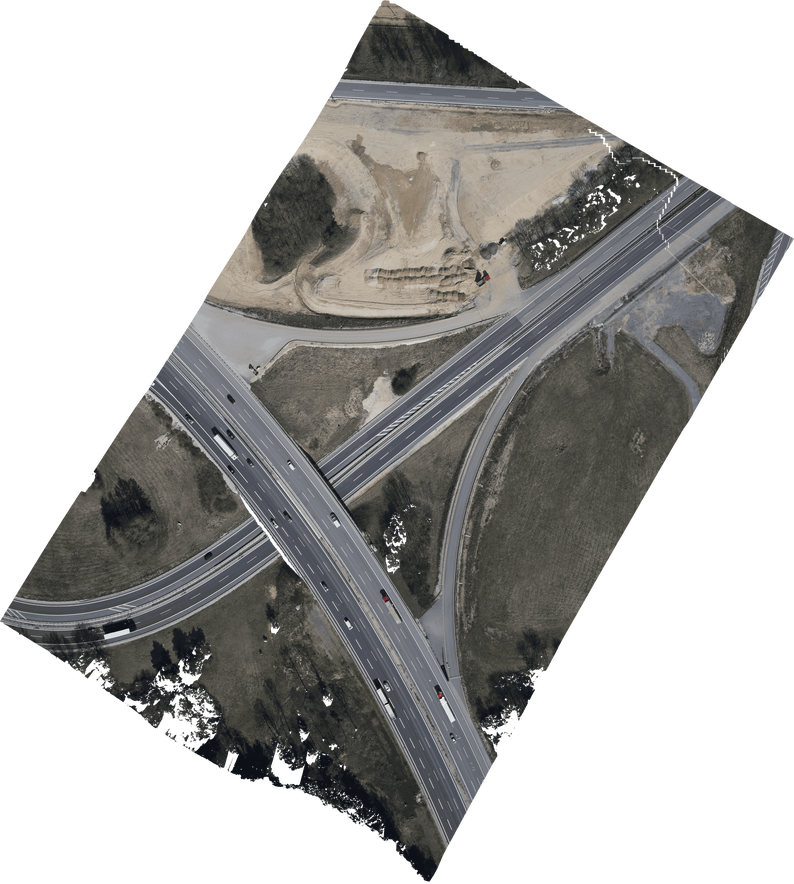
\includegraphics[width=0.45\textwidth]{OL1234_rsz.png}
    \caption{Orthorectified Image}
    \label{fig:OrthoImg}
  }
%  \hfill
%  \parbox{.3\linewidth}{
    \centering
    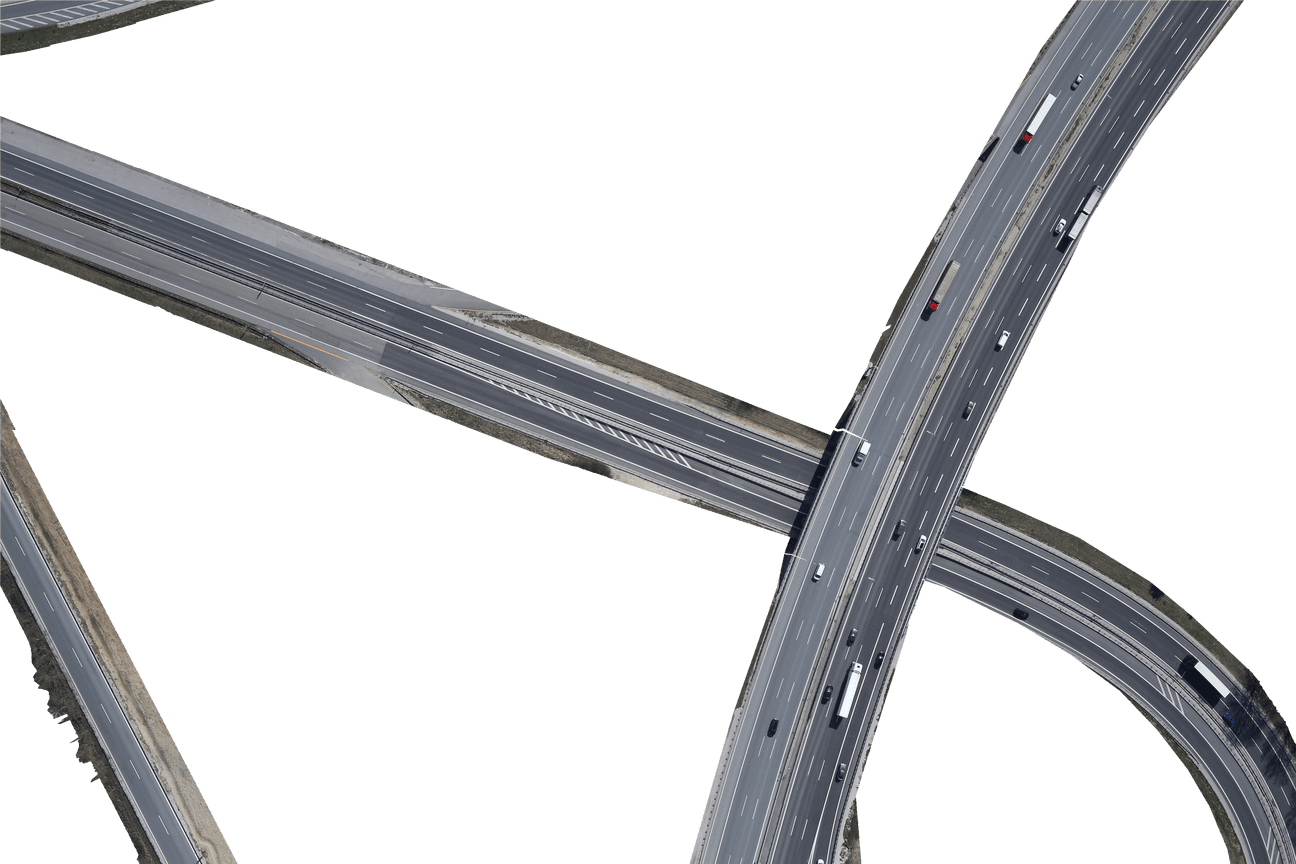
\includegraphics[width=0.7\textwidth]{ML1234_rsz.png}
    \caption{Masked Image}
    \label{fig:MaskedImg}
%  }
\end{figure}

\clearpage

%%%%%%%%%%%%%%%%%%%%%%%%%%%%%%%%%%%%%%%%%%%%%%%%%%%%%%%%
\section{Lane markings Extraction}
\label{sec:LineExtraction}

The principle to extract line features is to firstly derive the line direction for each pixel by using partial derivatives of a Gaussian smoothing kernel. Pixels that have a local maximum in the second directional derivative perpendicular to the line direction are marked as line points which are then linked and connected.

The $\sigma$ value for Gaussian smoothing is set to be 1.8 in this work to slightly suppress the noise. The extracted lines of length less than 30 pixels are rejected. Each accepted extracted line is rasterized as a set of points in image coordinates with sub-pixel precision.~\cref{fig:LineExtraction} shows the extracted lines on the original image.
% http://www.mvtec.com/doc/halcon/11/en/lines_gauss.html
\begin{figure}
  \centering
  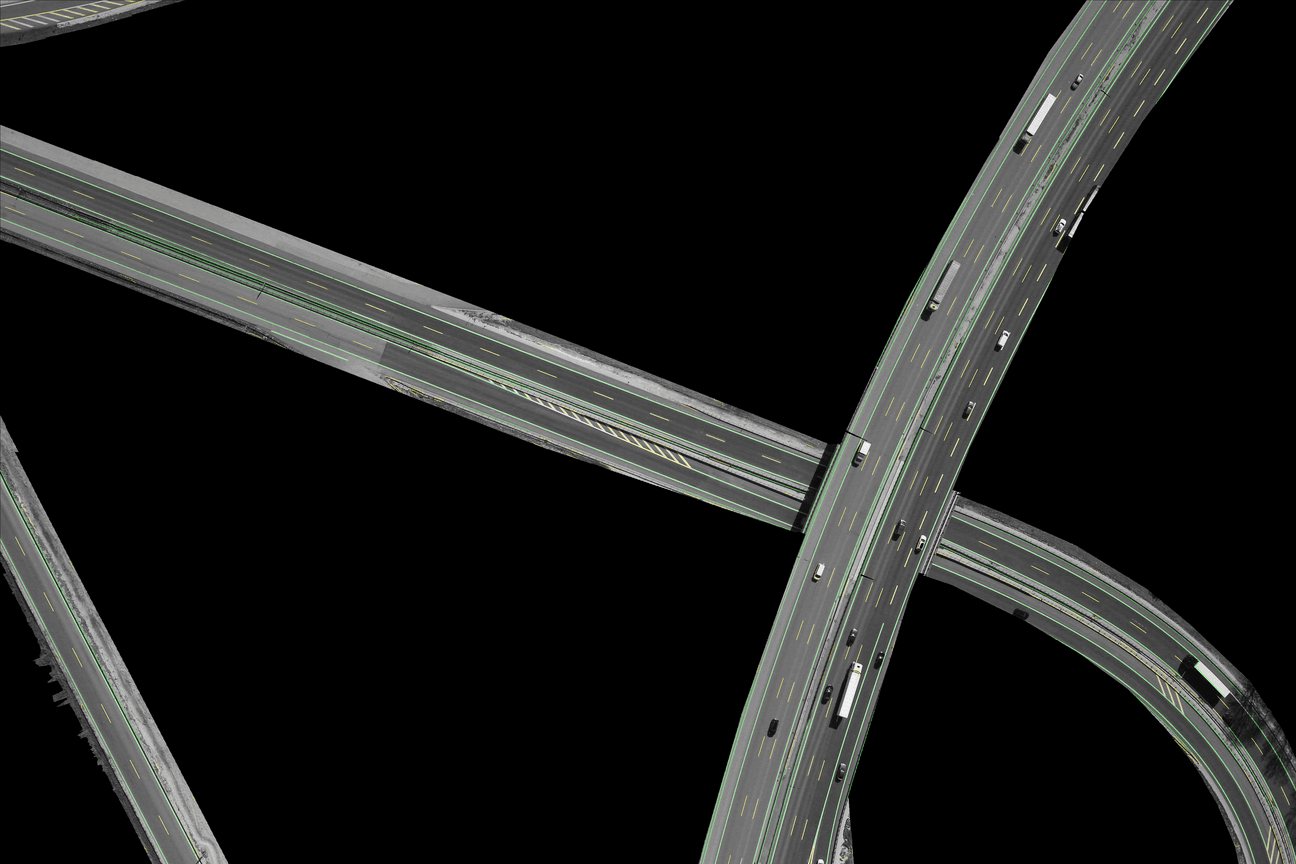
\includegraphics[width=0.7\textwidth]{ML1234_extlines_rsz.png}
  \caption{Lane markings Extraction. The extracted long lane-lines are marked in green and the dashed ones are in yellow.  Note that both cases are reconstructed into 3D with the same approach in the following sections; different colors here are only for illustration.}
  \label{fig:LineExtraction}
\end{figure}

%%%%%%%%%%%%%%%%%%%%%%%%%%%%%%%%%%%%%%%%%%%%%%%%%%%%%%%%
\section{Geometric Properties of Aerial Photographs}
\label{sec:Geometry}

This section describes the geometric model of the projection of 3D points into the image generated by a real camera. We first restrict the discussion in~\cref{subsec:Collinearity} to central perspective projection where the collinearity equation originate from. We then model deviations from this model, addressing real cameras with imperfect lenses, in~\cref{subsec:LensDistortion}.

\subsection{Collinearity Equations}
\label{subsec:Collinearity}
We assume frame photography, i.e. photographs exposed in one instant, and assume central projection model, i.e. cameras who have a single viewpoint and a planar sensor and being straight line-preserving. Collinearity indicates the condition that the image point (on the sensor plate of the camera), the observed point (on the object) and the projection center of the camera were aligned at the moment the picture was taken. Every measured point leads to two collinearity equations, describing transformations from object space to image coordinates:
\begin{equation} \label{eq:collinearity}
\begin{split}
x - x_0 = -c \dfrac {R_{11}(X-X_0) + R_{21}(Y-Y_0) + R_{31}(Z-Z_0)} {R_{13}(X-X_0) + R_{23}(Y-Y_0) + R_{33}(Z-Z_0)} \\
y - y_0 = -c \dfrac {R_{12}(X-X_0) + R_{22}(Y-Y_0) + R_{32}(Z-Z_0)} {R_{13}(X-X_0) + R_{23}(Y-Y_0) + R_{33}(Z-Z_0)}
\end{split}
\end{equation}
where\newline
$(x, y)$: image coordinates of the point \newline
$(x_0, y_0)$: image coordinates of principal point \newline
$c$: principal distance \newline
$(X, Y, Z)$: object coordinates of the point \newline
$(X_0, Y_0, Z_0)$: object coordinates of projection center \newline
$R_{11},...,R_{33}$: elements of the rotation matrix R (orthogonal 3$\times$3-matrix from object space to image space, with 3 independent angles $\omega$, $\phi$ and $\kappa$)

%The exterior orientations: $X_0$, $Y_0$, $Z_0$, $\omega$, $\phi$, $\kappa$ as well as the interior orientations: $x_0$, $y_0$, $c$ are the bundle-adjusted, known elements in this work.
%The image coordinates $x,y$ are the measurements.

\subsection{Lens Distortion Correction}
\label{subsec:LensDistortion}

As real cameras generally only approximate the perspective camera model, lens distortion correction can be additionally included in the collinearity model, attempting to correct the position of image features such that they obey the perspective model with sufficient accuracy.[W. Förstner et al. 2016] 
%(Varies models for lens distortion ...)
%A subset of a physical distortion model[] is chosen for...

A 6-parameter lens distortion model is chosen, with two radial symmetric distortion parameters $A_1$ and $A_2$, two asymmetric parameters $B_1$ and $B_2$, and a scaling $C1$ and an affine shearing parameter $C_2$. Assuming $x$ and $y$ to be the distorted image coordinates, the corrections $\Delta x$ and $\Delta y$ are then calculated by the following equations:
\begin{equation} \label{eq:LensDistortion}
\begin{split}
\Delta x &= x_p + A_1x_*(r^2-R_0^2) + A_2x_*(r^4-R_0^4) + B_1(r^2+2x_*^2) + B_22x_*y+C_2y \\
\Delta y &= y_p + A_1y  (r^2-R_0^2) + A_2y  (r^4-R_0^4) + B_1(r^2+2y^2)   + B_22x_*y
\end{split}
\end{equation}
with $r=\sqrt{x_*^2+y^2}$ and $x_*=\dfrac{x}{C_1}$. The undistorted image coordinates $x\prime$ and $y\prime$ are then calculated by $x\prime=x+\Delta x$ and $y\prime=y+\Delta y$. [F. Kurz et al. 2012] 

%This allows us to reconstruct the viewing rays from the corresponding set of image points.


%%%%%%%%%%%%%%%%%%%%%%%%%%%%%%%%%%%%%%%%%%%%%%%%%%%%%%%%
\section{Line Fitting}
\label{sec:LineFitting}

Line fitting is the process of constructing a infinite straight line that has the best fit to a 2D dataset. One of the approaches is linear regression which attempts to model the relationship between two variables by fitting a linear equation to observed data. % [www.stat.yale.edu/Courses/1997-98/101/linreg.htmf]
Additional least-squares (LS) models are commonly used for regression by means of minimization of sum of squared residuals.

In the case of simple linear regression as presented in~\cref{subsec:LinearRegression}, the independent variable $x$ is error free, inconsistencies are only for the dependent variable $y$. Geometrically it means that the vertical distances from observed data to the fitted line is minimized. To minimize the sum of squared perpendicular distances from the data points to the regression line, a LS mixed model is derived in ~\cref{subsec:MixedModel} to perform orthogonal regression.

For a later combination with collinearity equations \eqref{eq:collinearity}, we aim to fit the line equation in two-point form to the extracted lines produced in~\cref{sec:LineExtraction} (in forms of sets of points in image coordinates). For such purpose, a non-linear LS adjustment model is derived in~\cref{subsec:NonLinear}. 


\subsection{Linear Regression}
\label{subsec:LinearRegression}

Given a data set $\{x_i,y_i\}^n_{i=1}$ of $n$ points on a 2D plane, a linear regression model assumes that the relationship between the dependent variable $y_i$ and the regressors $x_i$ is linear. This relationship is modeled through a error variable $e_{y_i}$--- an unobserved random variable that adds noise to the linear relationship between the dependent variable and regressors.
Thus the model takes the form:
\begin{equation} \label{eq:SimpleLinearRegression}
y_i - e_{y_i} = a_0 + a_1x_i
\end{equation}
where $a_0$ and $a_1$ are the regression coefficients.
%https://en.wikipedia.org/wiki/Linear_regression#Assumptions


\subsection{Mixed Model (Gauss-Helmert Model)}
\label{subsec:MixedModel}

In the case with inconsistencies $e_{x_i}$ and $e_{y_i}$ in both observations $x_i$ and $y_i$, A-model with pseudo observation equations can be adopted and is formulated:
\begin{equation} \label{eq:MixModel1}
y_i - e_{y_i} = a_0 + a_1(x_i-e_{x_i}) = a_0 + a_1\bar{x_i}
\end{equation}
\begin{equation} \label{eq:MixModel2}
x_i-e_{x_i} = \bar{x_i}
\end{equation}

In the A-model, every observation is either a linear or a non-linear function of all unknown quantities. In contrast, in the B-model no unknown parameter exist and there are linear or non-linear relationships between the observations [F. Krumm]. As \eqref{eq:MixModel1} describes the relationship between observations and unknowns and \eqref{eq:MixModel2} describes the relationship between observations, the whole set is known as the mixed model or Gauss-Helmert model.




\subsection{Non-linear LS Model}
\label{subsec:NonLinear}

Line Equation in two-point form:
\begin{equation} \label{eq:LineInTwoPointForm}
y-y_1 = \dfrac{(y_2-y_1)}{(x_2-x_1)}\times(x-x_1)
\end{equation}
where two points $(x_1,y_1)$ and $(x_2,y_2)$ define the infinite line with $x_2\neq x_1$ and $(x,y)$ is any point on the line.

Let the unknown image coordinates of the start- and endpoints of a line be $(x_1,y_1)$ and $(x_2,y_2)$, and the observations $\{x_i,y_i\}^n_{i=1}$. Rewriting \eqref{eq:LineInTwoPointForm} in the form of \eqref{eq:MixModel1} gives:
\begin{equation} %\label{eq:2.3}
y_i - e_{y_i}= (y_1-\dfrac{(y_2-y_1)}{(x_2-x_1)}\times x_1) + \dfrac{(y_2-y_1)}{(x_2-x_1)}\times x_i
\end{equation}
% which can be further rewritten:

% % %
%forms the observation equation
%The observations $y_i$ are non-linear functions of all unknown quantities.
%Taylor expansion...(local linear approximation)
%the linear equation can also be expanded

%\clearpage
%%%%%%%%%%%%%%%%%%%%%%%%%%%%%%%%%%%%%%%%%%%%%%%%%%%%%%%%
\section{LS Adjustment for 3D lane markings reconstruction}
\label{sec:LSadj}

At the moment an aerial image ...
In this section, the

\subsection{constraints}
\label{subsec:}

% % %
C matrix
D matrix

\subsection{LS Adjustment with Constraints}
\label{sec:}
Line fitting in image space with unknowns in object coordinates


% % %
derive matrices
extended normal equation matrix N*


%%%%%%%%%%%%%%%%%%%%%%%%%%%%%%%%%%%%%%%%%%%%%%%%%%%%%%%%
\section{Line Projection on DSM}
\label{sec:LineProjectionOnDSM}

Given image coordinates $(x,y)$ of a point and the (bundle-adjusted) image orientations, there is still one degree of freedom in collinearity equation system Equa. on solving object coordinates $(X,Y,Z)$. Combined with the usage of DSM, who provides an initial height information given a position $(X,Y)$, the corresponding object coordinates can be solved iteratively.

With the following work flow:

pseudo code:

%x,y = a set of points (detected line);		// unit: [pixel], in image coordinates
%Z_ini = 500;						// unit: [meter], in world coordinates
%while( ( Z_new – Z_ini ) < convergentthreshold )
%	(X,Y) = camera.img2geo(x,y,Z_ini);	// X,Y in world coordinates
%	Z_new = DSM.Get_height(X,Y);		// Z_new in world coordinates
%end
%return (X,Y,Z_new);

%\begin{Algorithmus} 
%\caption{Line Projection on DSM}
%\label{alg:LineProjectionOnDSM}
%\begin{algorithmic}
%\Procedure{Sample}{$a$,$v_e$}
%  \State $\mathsf{parentHandled} \gets (a = \mathsf{process}) \lor \mathsf{visited}(a'), (a',c,a) \in \mathsf{HR}$
%  \State \Comment $(a',c'a) \in \mathsf{HR}$ denotes that $a'$ is the parent of $a$
%  \If{$\mathsf{parentHandled}\,\land(\mathcal{L}_\mathit{in}(a)=\emptyset\,\lor\,\forall l \in %\mathcal{L}_\mathit{in}(a): \mathsf{visited}(l))$}
%    \State $\mathsf{visited}(a) \gets \text{true}$
%    \State $\mathsf{writes}_\circ(a,v_e) \gets
%    \begin{cases}
%      \mathsf{joinLinks}(a,v_e)                & \abs{\mathcal{L}_\mathit{in}(a)} > 0\\
%      \mathsf{writes}_\circ(p,v_e)             & \exists p: (p,c,a) \in \mathsf{HR}\\
%      (\emptyset, \emptyset, \emptyset, false) & \text{otherwise}
%    \end{cases}
%  \EndIf
%\EndProcedure
%\end{algorithmic}
%\end{Algorithmus}













Considering that X,Y have continuous numerical values whereas the DSM is raster (discrete), bilinear interpolation is adopted in this work.

% % %
to provide the initial approximation for non-linear LS adj





%%%%%%%%%%%%%%%%%%%%%%%%%%%%%%%%%%%%%%%%%%%%%%%%%%%%%%%%
\section{Line Grouping}
\label{sec:}





%\begin{equation}\label{eq:test}
%a = b + c.
%\end{equation}

%\begin{equation}
%a = b + c. \tag{\ref{eq:test} revisited}
%\end{equation}



